\documentclass[11pt,fleqn]{article}

\setlength {\topmargin} {-.15in}
\setlength {\textheight} {8.6in}

\usepackage{amsmath}
\usepackage{amssymb}
\usepackage{color}
\usepackage{tikz}
\usetikzlibrary{automata,positioning,arrows}
\usepackage{diagbox}
\usepackage{stackrel}
\begin{document}


\textbf{1.5.14:} Weighted quick-union by height. Develop a UF implementation that uses the
same basic strategy as weighted quick-union but keeps track of tree height and always
links the shorter tree to the taller one. Prove a $logarithmic$ $upper$ $bound$ on the height
of the trees for N sites with your algorithm.\\

\textbf{Overview:} Max height will have a total of $logN$ height. Initially each node seperate and has height of 1. 2 arrays are required. One will be to keep track of the height. The other will keep track of parent/root nodes.\\

\textbf{Pseudocode below:}\\

\begin{center}
	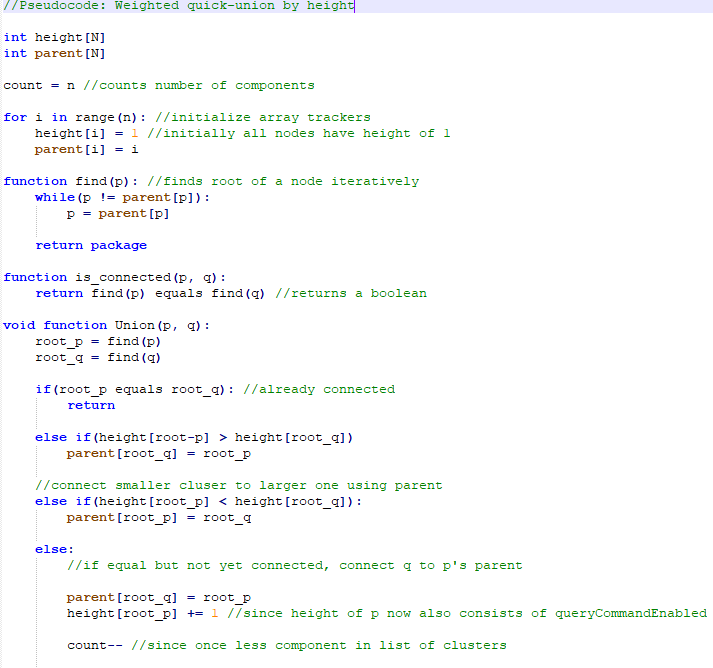
\includegraphics[scale = 1]{1.5.14.png}
	\end{center}

\end{document}
